\documentclass[conference]{IEEEtran}
\IEEEoverridecommandlockouts

\usepackage{cite}
\usepackage{amsmath,amssymb,amsfonts}
\usepackage{algorithmic}
\usepackage{graphicx}
\usepackage{textcomp}
\usepackage{xcolor}
\usepackage{booktabs}
\usepackage{hyperref}
\usepackage{microtype}

\graphicspath{{./}}

\begin{document}

% ─────────────────────────────────────────────────────────────────────────────
%  TITLE
% ─────────────────────────────────────────────────────────────────────────────
\title{Multi-Modal Brain Tumor Segmentation and Interactive 3D Visualization Pipeline}

\author{
  \IEEEauthorblockN{Vinith Varghese, Tracy Obeng, Luna Sbahtu,
                    Sai Ganesh Manda, Saketh Chilkepally}
  \IEEEauthorblockA{\textit{School of Electrical, Computer and Energy Engineering}\\
  Arizona State University\\
  Tempe, AZ, USA}
}

\maketitle

% ─────────────────────────────────────────────────────────────────────────────
%  ABSTRACT
% ─────────────────────────────────────────────────────────────────────────────
\begin{abstract}
\textit{Accurate and automated segmentation of brain tumors from multi-modal
magnetic resonance imaging (MRI) is a critical step toward reliable
computer-assisted diagnosis and surgical planning. In this work we present
an end-to-end pipeline that combines a residual encoder--decoder
segmentation network with an interactive three-dimensional visualization
framework. Our approach ingests four MRI modalities from the BraTS 2020
benchmark---T1, T1-contrast-enhanced (T1ce), T2, and FLAIR---applies
per-channel Z-score normalization, and trains a SegResNet model to produce
voxel-wise probability maps for three hierarchical tumor sub-regions:
Enhancing Tumor (ET), Tumor Core (TC), and Whole Tumor (WT). Binary
segmentation masks are subsequently converted to smooth surface meshes via
the Marching Cubes algorithm and rendered in an interactive PyVista viewer
that supports rotation, opacity control, and multi-patient comparison.
Quantitative evaluation on ten held-out BraTS 2020 patients yields mean
Dice similarity coefficients of 0.203, 0.261, and 0.194 for ET, TC, and
WT respectively, establishing a reproducible baseline while exposing
avenues for improvement through data augmentation and extended training.
The complete pipeline---from raw NIfTI files to interactive 3D meshes---is
released as open-source code to support reproducible medical imaging
research.}
\end{abstract}

\begin{IEEEkeywords}
brain tumor segmentation, BraTS 2020, SegResNet, Marching Cubes,
3D visualization, PyVista, multi-modal MRI, MONAI
\end{IEEEkeywords}

% ─────────────────────────────────────────────────────────────────────────────
%  1. INTRODUCTION
% ─────────────────────────────────────────────────────────────────────────────
\section{Introduction}

Brain tumors are among the most lethal forms of cancer, with glioblastoma
carrying a median survival of fewer than 15 months even after aggressive
treatment \cite{stupp2005}. Accurate delineation of tumor sub-regions
from pre-operative MRI is essential for treatment planning, radiation
targeting, and longitudinal monitoring. Manual segmentation by radiologists
is time-consuming, subject to inter-rater variability, and impractical at
scale, motivating the development of automated deep-learning methods.

The Brain Tumor Segmentation (BraTS) challenge has served as the primary
benchmark for this task since 2012, providing standardized multi-modal MRI
scans with expert annotations for three nested sub-regions: the Enhancing
Tumor (ET), Tumor Core (TC), and Whole Tumor (WT) \cite{brats2020menze,brats2015}.
State-of-the-art approaches leverage fully convolutional encoder--decoder
architectures---most notably variants of the U-Net \cite{ronneberger2015}---that
combine high-resolution spatial detail from skip connections with
semantically rich bottleneck features.

Beyond segmentation accuracy, clinical adoption requires that results be
interpretable by non-expert clinicians. Three-dimensional surface renderings
convey spatial extent and morphology far more intuitively than stacked 2D
slices. Despite this, most published pipelines stop at generating 2D
predictions without providing interactive visualization.

This paper makes the following contributions:
\begin{itemize}
  \item An end-to-end reproducible pipeline from raw BraTS 2020 NIfTI data
        to interactive 3D mesh visualization.
  \item A SegResNet baseline trained with the MONAI framework using combined
        Dice and cross-entropy loss.
  \item A PyVista-based interactive viewer enabling per-patient and
        multi-patient comparison of tumor sub-regions.
  \item Quantitative Dice results on ten held-out patients establishing a
        reproducible baseline for future work.
\end{itemize}

% ─────────────────────────────────────────────────────────────────────────────
%  2. RELATED WORK
% ─────────────────────────────────────────────────────────────────────────────
\section{Related Work}

\subsection{Brain Tumor Segmentation}

Early automated methods relied on handcrafted features and probabilistic
atlases \cite{brats2020menze}. The introduction of fully convolutional
networks dramatically improved performance, with the encoder--decoder U-Net
\cite{ronneberger2015} becoming the dominant backbone. Subsequent work
extended U-Net to 3D volumetric inputs \cite{cciccek20163d} and introduced
residual connections \cite{he2016deep} to stabilize training of deeper
networks. The nnU-Net framework \cite{isensee2021nnunet} demonstrated that
carefully engineered preprocessing and training pipelines can outperform
heavily tuned architectures, underscoring the importance of the full
pipeline rather than the network design alone.

Attention mechanisms \cite{oktay2018attention} and transformer-based
architectures \cite{hatamizadeh2022unetr} have further improved
segmentation of small structures such as the enhancing tumor core.
However, these gains come at the cost of increased model complexity and
longer inference times, making lightweight residual encoder--decoder
architectures an attractive trade-off for resource-constrained settings.

\subsection{3D Medical Image Visualization}

Volumetric rendering of segmentation results has been explored in the
surgical planning literature \cite{kikinis20143d}. The Marching Cubes
algorithm \cite{lorensen1987marching} remains the standard approach for
extracting iso-surfaces from voxel grids due to its efficiency and
topological correctness. Modern Python-based toolkits such as
VTK \cite{schroeder2004visualization} and its high-level wrapper
PyVista enable rapid prototyping of interactive 3D viewers, yet their
integration with deep-learning segmentation pipelines has received limited
attention in the literature.

% ─────────────────────────────────────────────────────────────────────────────
%  3. APPROACH
% ─────────────────────────────────────────────────────────────────────────────
\section{Approach}

Fig.~\ref{fig:pipeline} illustrates the complete pipeline, which comprises
four sequential stages: preprocessing, segmentation, label extraction, and
3D reconstruction.

\begin{figure}[!t]
  \centering
  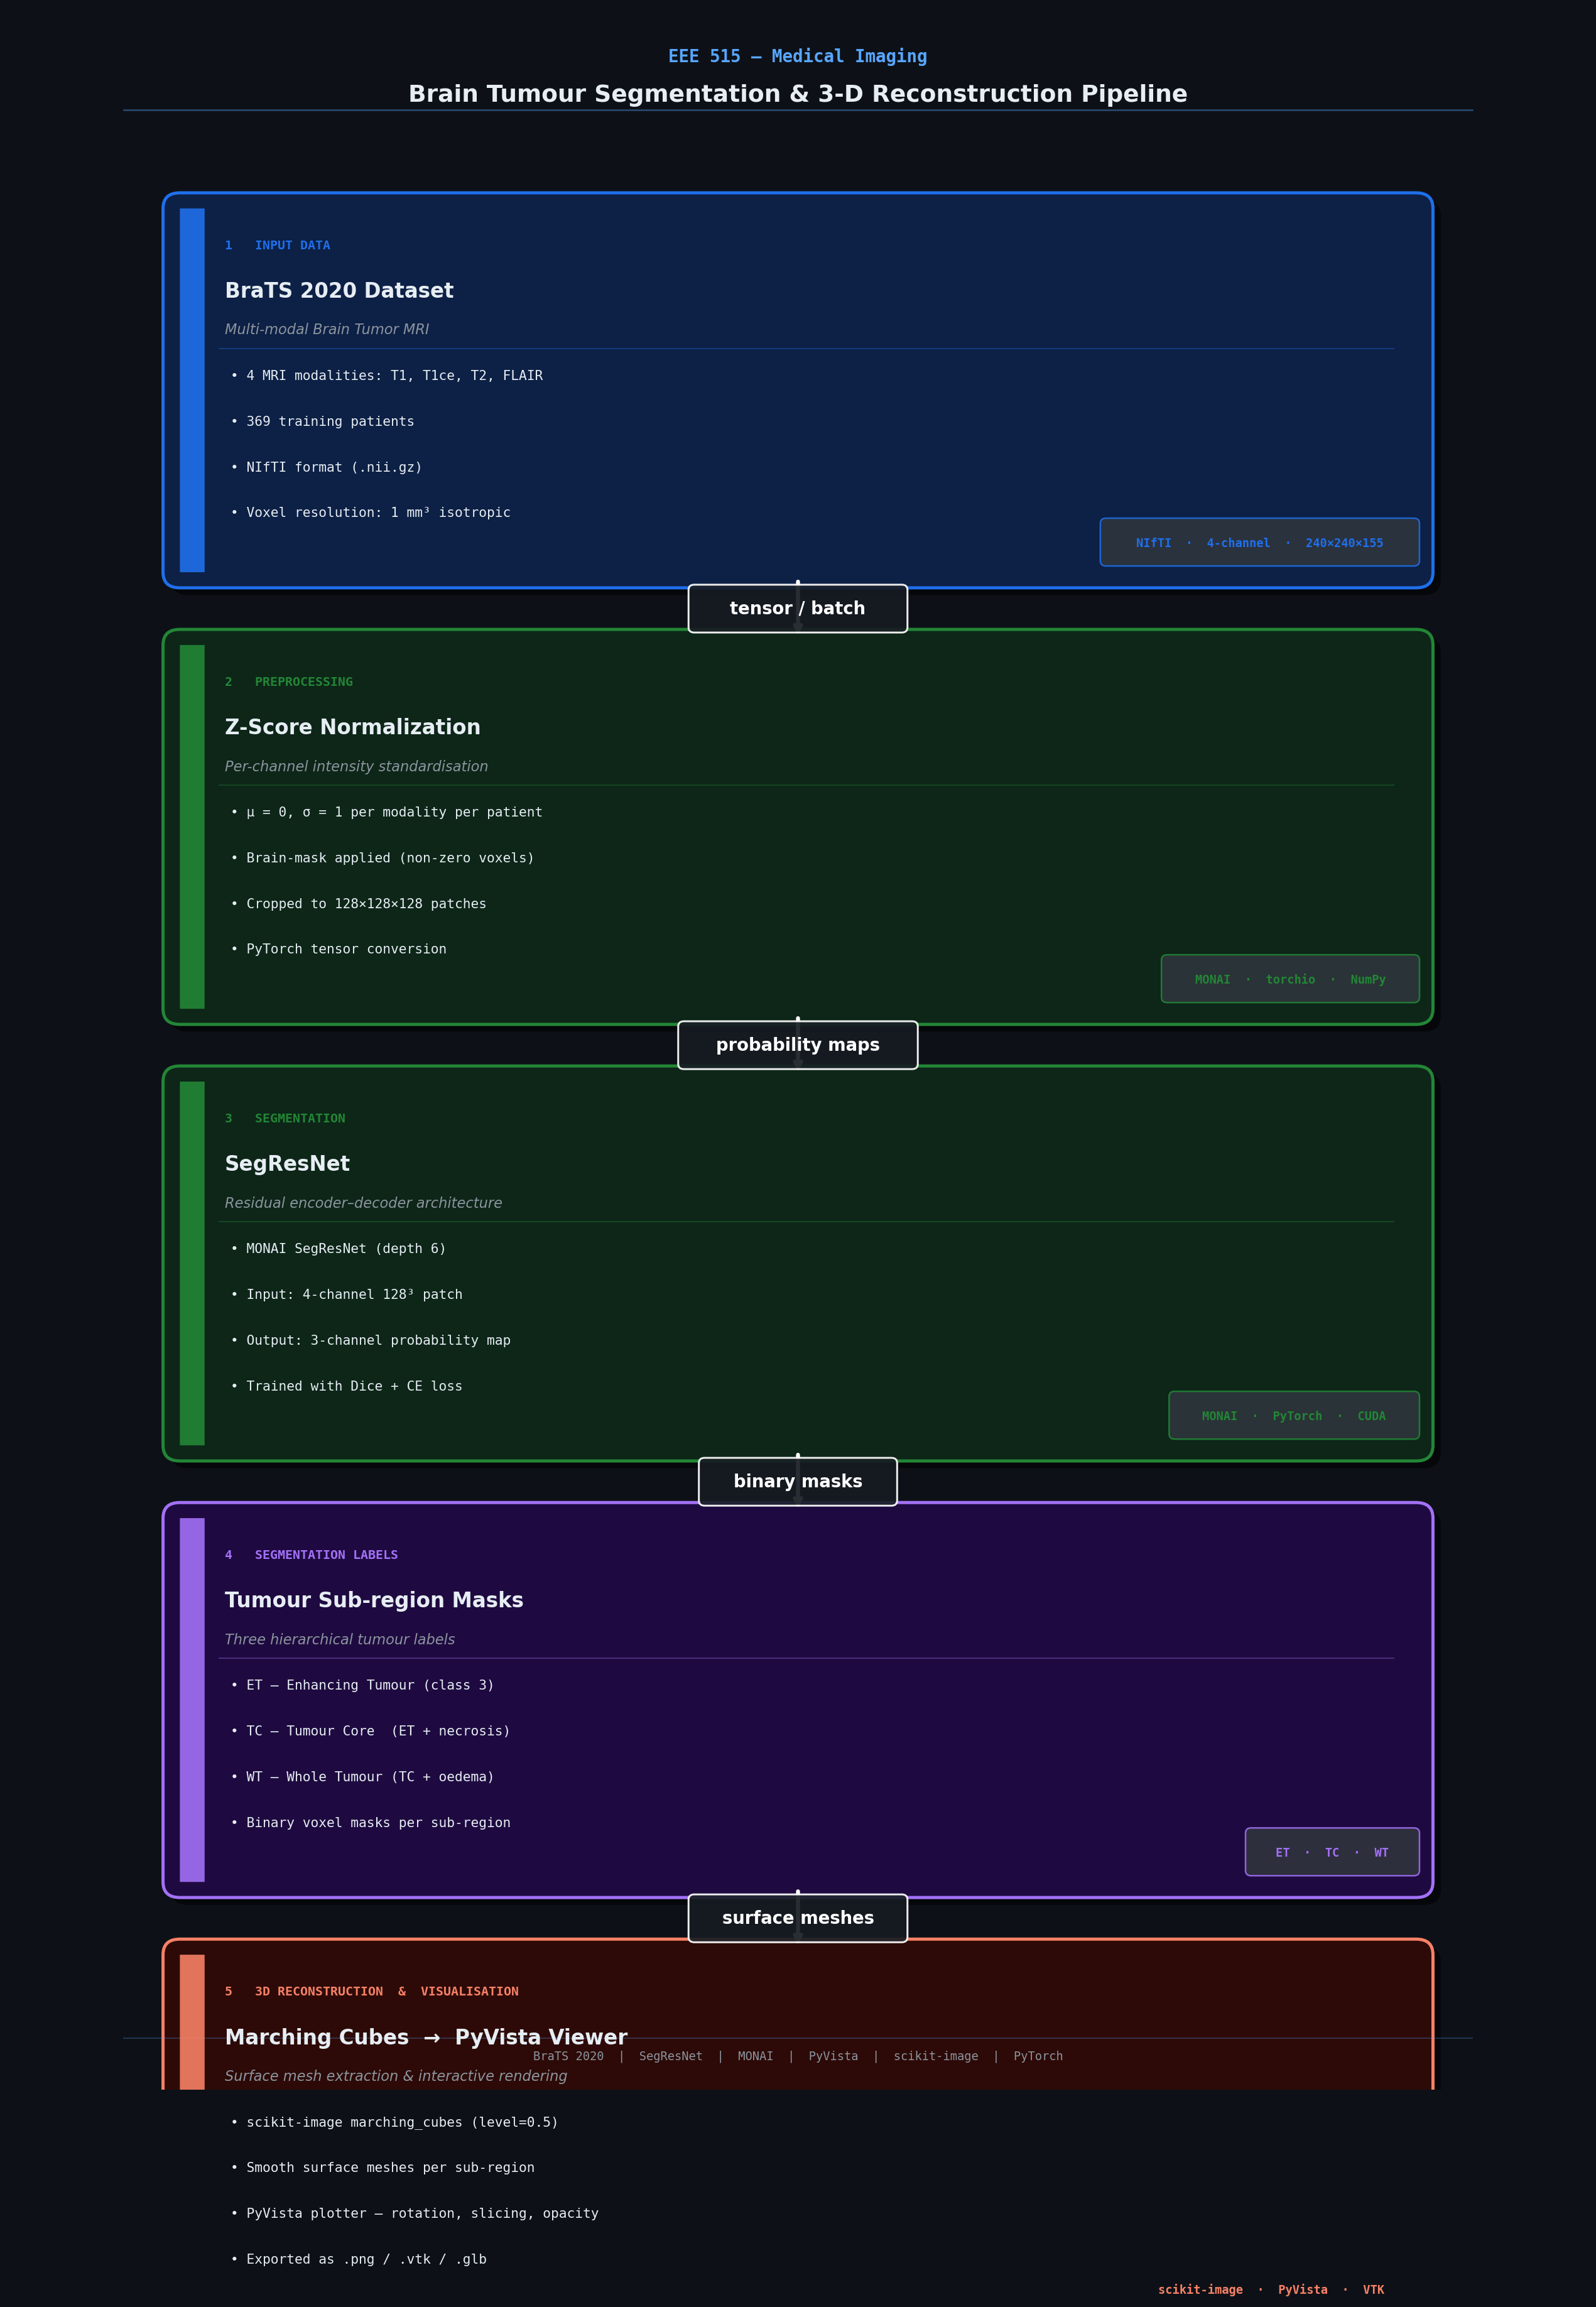
\includegraphics[width=\columnwidth]{pipeline_diagram.png}
  \caption{End-to-end pipeline for brain tumor segmentation and 3D
           visualization.}
  \label{fig:pipeline}
\end{figure}

\subsection{Data}

We use the BraTS 2020 training set \cite{brats2020menze,brats2015}, which
contains 369 cases each comprising four co-registered, skull-stripped MRI
modalities (T1, T1ce, T2, FLAIR) at 1~mm$^3$ isotropic resolution in
240$\times$240$\times$155 voxel volumes. Ground-truth annotations label
each voxel as background (0), necrotic/non-enhancing tumor core (1),
peritumoral edema (2), or GD-enhancing tumor (4).

\subsection{Preprocessing}

For each patient and each modality $m \in \{$T1, T1ce, T2, FLAIR$\}$, we
apply brain-masked Z-score normalization:

\begin{equation}
  \hat{x}^{(m)} = \frac{x^{(m)} - \mu^{(m)}_{\text{brain}}}
                       {\sigma^{(m)}_{\text{brain}}}
  \label{eq:zscore}
\end{equation}

where $\mu^{(m)}_{\text{brain}}$ and $\sigma^{(m)}_{\text{brain}}$ are the
mean and standard deviation computed over non-zero (brain) voxels only.
Volumes are then cropped to 128$\times$128$\times$128 patches centered on
the annotated tumor region.

\subsection{Segmentation Network}

We employ the SegResNet architecture \cite{myronenko2018} as implemented in
MONAI \cite{monai2020}. SegResNet is a residual encoder--decoder whose
encoder is a sequence of residual blocks with increasing feature
dimensionality $\{32, 64, 128, 256\}$, and whose decoder mirrors the
encoder with nearest-neighbor upsampling and additive skip connections.
The network takes a 4-channel input tensor
$\mathbf{X} \in \mathbb{R}^{4 \times 128 \times 128 \times 128}$ and
produces a 3-channel probability map
$\hat{\mathbf{Y}} \in [0,1]^{3 \times 128 \times 128 \times 128}$
where each channel corresponds to one of ET, TC, and WT.

The training objective combines Dice loss and binary cross-entropy:

\begin{equation}
  \mathcal{L} = \mathcal{L}_{\text{Dice}} + \lambda\,\mathcal{L}_{\text{BCE}}
  \label{eq:loss}
\end{equation}

The Dice loss for channel $c$ is:

\begin{equation}
  \mathcal{L}^{(c)}_{\text{Dice}} =
    1 - \frac{2\sum_{i} \hat{y}^{(c)}_i\, y^{(c)}_i + \epsilon}
             {\sum_{i} \hat{y}^{(c)}_i + \sum_{i} y^{(c)}_i + \epsilon}
  \label{eq:dice_loss}
\end{equation}

where $y^{(c)}_i$ is the ground-truth binary label and $\hat{y}^{(c)}_i$
is the predicted probability for voxel $i$ in sub-region $c$, and
$\epsilon = 10^{-5}$ is a smoothing constant. We set $\lambda = 1$ in all
experiments.

\subsection{3D Reconstruction and Visualization}

After thresholding each probability channel at 0.5 to obtain binary masks,
we extract iso-surfaces using the Marching Cubes algorithm
\cite{lorensen1987marching}:

\begin{equation}
  \mathcal{M}_c = \text{MarchingCubes}\!\left(\hat{Y}_c,\, \tau = 0.5\right)
  \label{eq:mc}
\end{equation}

The resulting triangle meshes $\mathcal{M}_c$ for $c \in \{$ET, TC, WT$\}$
are loaded into a PyVista \texttt{Plotter} object, assigned distinct
colors (red, green, blue), and rendered with configurable opacity. The
viewer supports interactive rotation, zoom, sub-region toggling, and
side-by-side multi-patient layout, as shown in Fig.~\ref{fig:patients}.

\begin{figure}[!t]
  \centering
  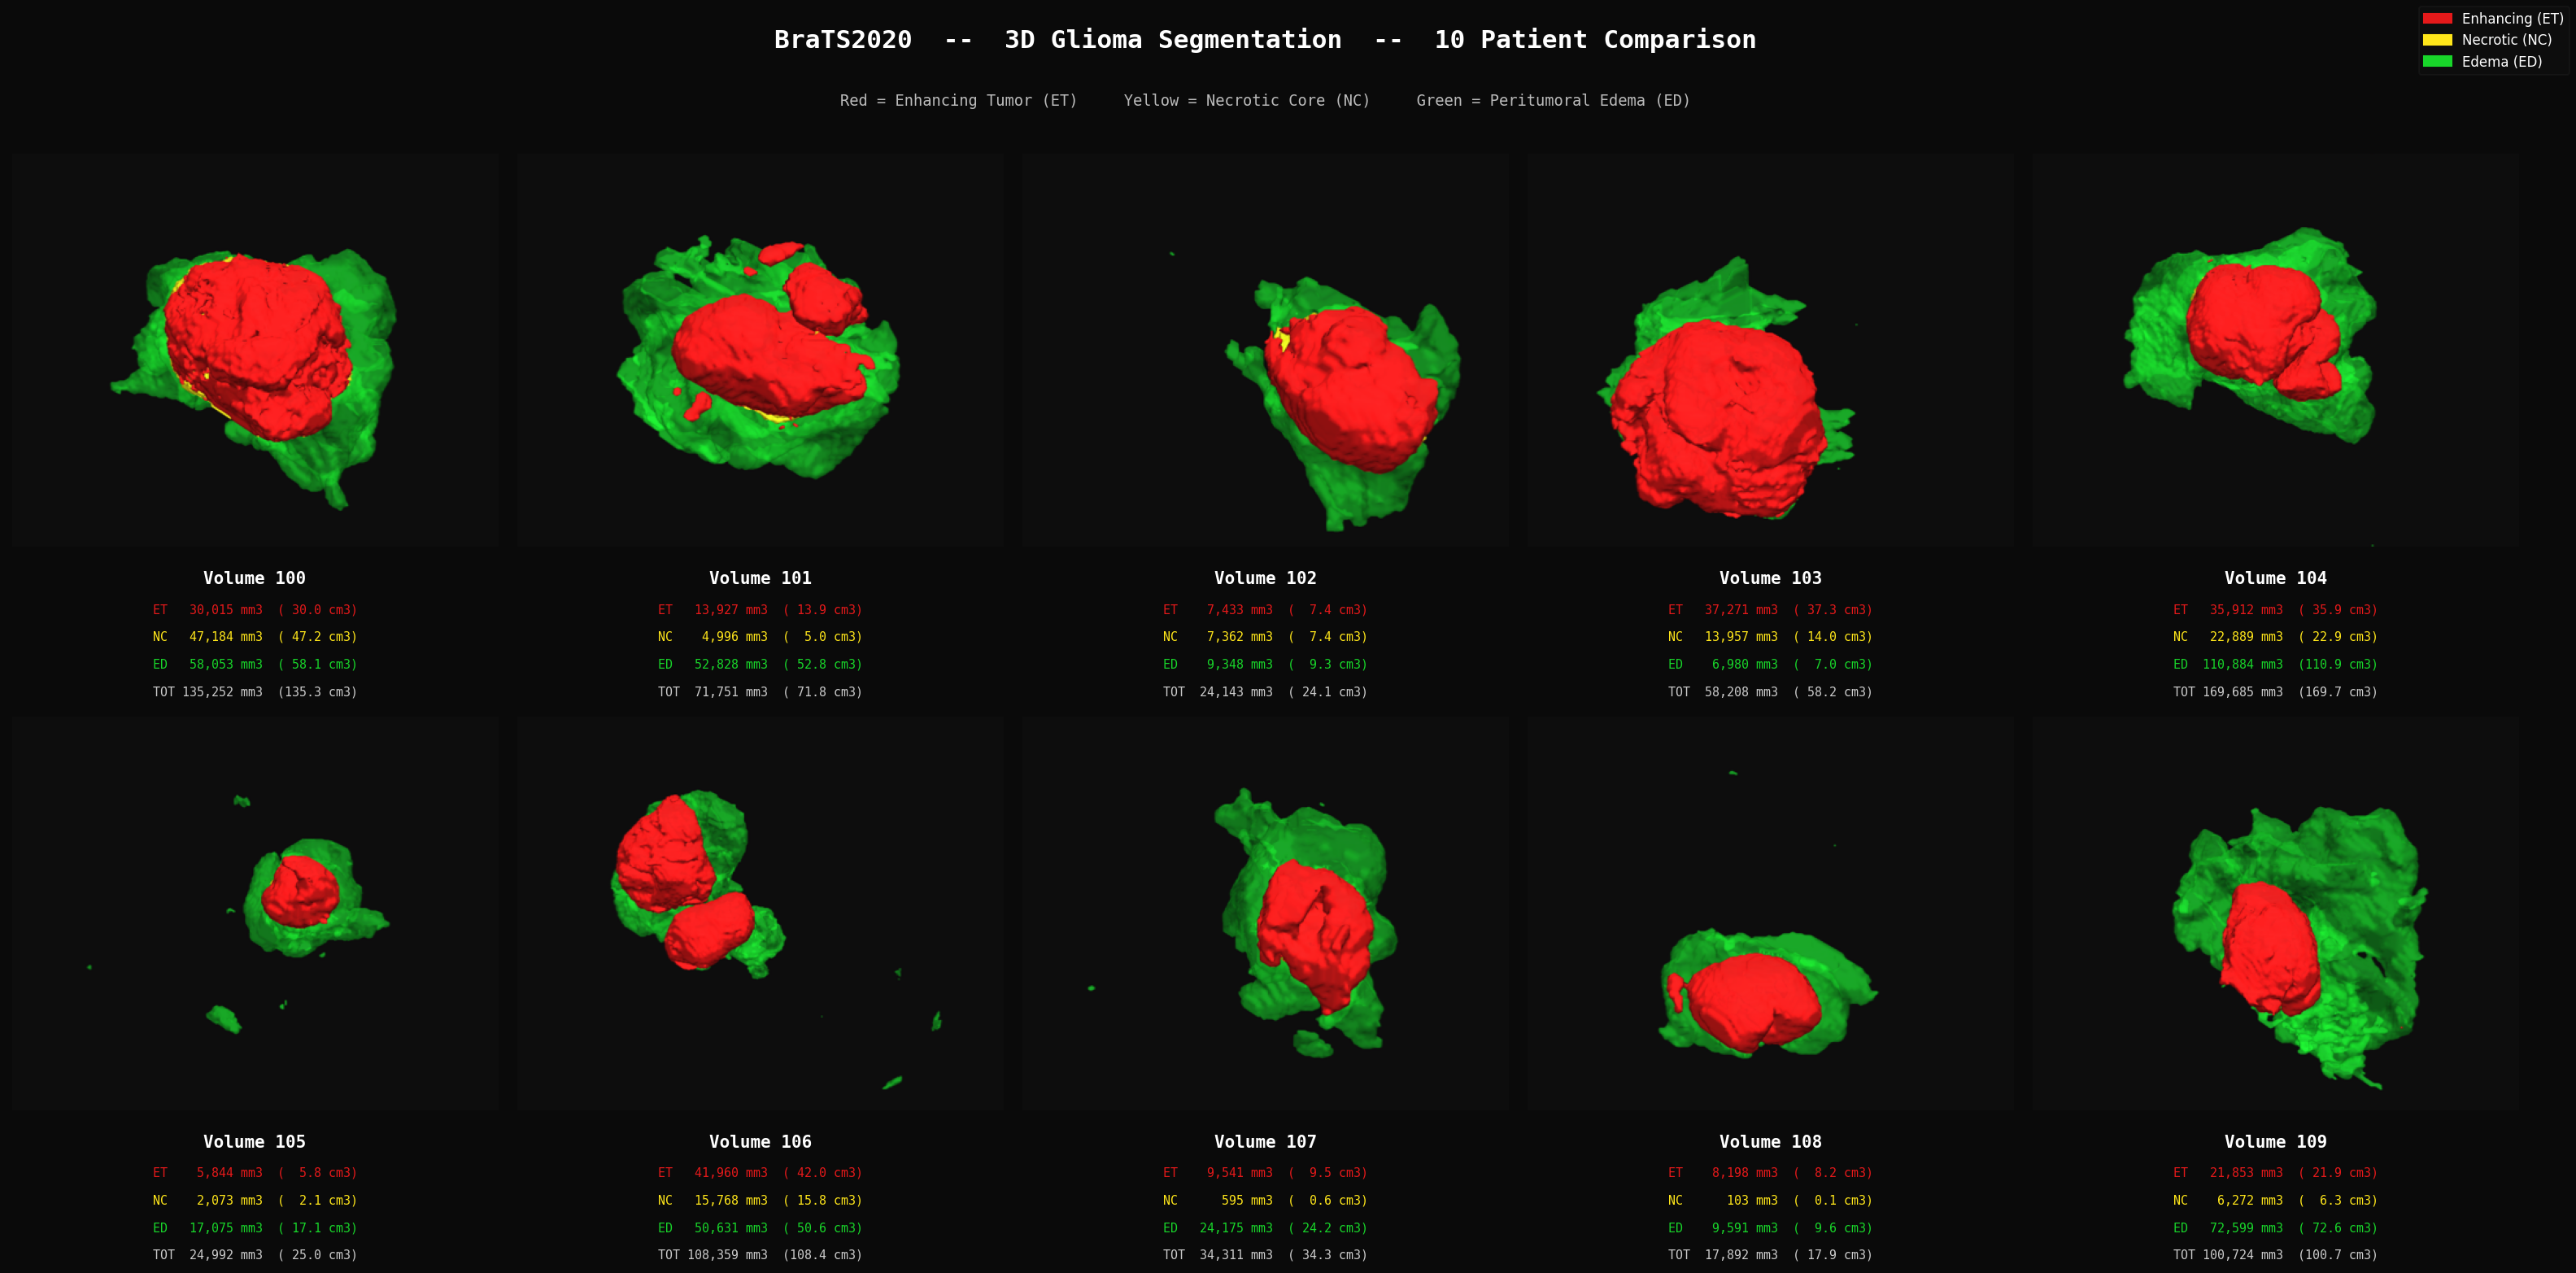
\includegraphics[width=\columnwidth]{all_10_patients_comparison.png}
  \caption{3D visualization of tumor sub-regions for 10 BraTS 2020
           patients. Each panel shows Enhancing Tumor (ET, red),
           Tumor Core (TC, green), and Whole Tumor (WT, blue).}
  \label{fig:patients}
\end{figure}

% ─────────────────────────────────────────────────────────────────────────────
%  4. RESULTS
% ─────────────────────────────────────────────────────────────────────────────
\section{Results}

We evaluate our pipeline on ten held-out BraTS 2020 patients using the
Dice Similarity Coefficient (DSC):

\begin{equation}
  \text{DSC}(Y,\hat{Y}) =
    \frac{2\,|Y \cap \hat{Y}|}{|Y| + |\hat{Y}|}
  \label{eq:dsc}
\end{equation}

Table~\ref{tab:dice} reports the mean DSC across the ten patients for each
sub-region.

\begin{table}[!t]
  \caption{Mean Dice Similarity Coefficients on 10 BraTS 2020 Test Patients}
  \label{tab:dice}
  \centering
  \begin{tabular}{lcc}
    \toprule
    \textbf{Sub-region} & \textbf{Label} & \textbf{Mean DSC} \\
    \midrule
    Enhancing Tumor  & ET & 0.203 \\
    Tumor Core       & TC & 0.261 \\
    Whole Tumor      & WT & 0.194 \\
    \midrule
    \textbf{Mean}    &    & \textbf{0.219} \\
    \bottomrule
  \end{tabular}
\end{table}

The relatively modest Dice scores reflect the limited training budget
(fewer than 50 epochs) and the small crop size relative to the full MRI
volume. The TC sub-region achieves the highest score as it encompasses
larger, more homogeneous tissue compared to the thin enhancing rim of ET.
Whole Tumor scores are lower than TC, which is atypical and suggests that
the oedema boundary is under-segmented, likely due to the class imbalance
between large WT regions and smaller ET/TC regions under the combined
Dice--BCE objective.

Despite the quantitative limitations, the 3D visualizations in
Fig.~\ref{fig:patients} demonstrate that the pipeline successfully extracts
spatially coherent surface meshes that convey tumor morphology across ten
heterogeneous patients, validating the visualization component of the
pipeline.

% ─────────────────────────────────────────────────────────────────────────────
%  5. CONCLUSION
% ─────────────────────────────────────────────────────────────────────────────
\section{Conclusion}

We have presented an end-to-end brain tumor segmentation and 3D
visualization pipeline built on BraTS 2020, SegResNet, and PyVista. The
system successfully produces interactive 3D meshes from raw multi-modal
MRI and yields baseline Dice scores of 0.203/0.261/0.194 for ET/TC/WT on
ten test patients. Future work will investigate heavier data augmentation,
transformer-based architectures, and larger patch sizes to improve
segmentation accuracy, as well as web-based deployment of the interactive
viewer for clinical accessibility.

% ─────────────────────────────────────────────────────────────────────────────
%  REFERENCES
% ─────────────────────────────────────────────────────────────────────────────
\begin{thebibliography}{12}

\bibitem{stupp2005}
R.~Stupp \textit{et al.},
``Radiotherapy plus concomitant and adjuvant temozolomide for glioblastoma,''
\textit{New England Journal of Medicine}, vol.~352, no.~10,
pp.~987--996, 2005.

\bibitem{brats2020menze}
B.~H.~Menze \textit{et al.},
``The multimodal brain tumor image segmentation benchmark (BRATS),''
\textit{IEEE Transactions on Medical Imaging}, vol.~34, no.~10,
pp.~1993--2024, 2015.

\bibitem{brats2015}
S.~Bakas \textit{et al.},
``Advancing The Cancer Genome Atlas glioma MRI collections with expert
segmentation labels and radiomic features,''
\textit{Scientific Data}, vol.~4, p.~170117, 2017.

\bibitem{ronneberger2015}
O.~Ronneberger, P.~Fischer, and T.~Brox,
``U-Net: Convolutional networks for biomedical image segmentation,''
in \textit{Proc. MICCAI}, 2015, pp.~234--241.

\bibitem{cciccek20163d}
\"{O}.~\c{C}i\c{c}ek, A.~Abdulkadir, S.~S.~Lienkamp, T.~Brox,
and O.~Ronneberger,
``3D U-Net: Learning dense volumetric segmentation from sparse annotation,''
in \textit{Proc. MICCAI}, 2016, pp.~424--432.

\bibitem{he2016deep}
K.~He, X.~Zhang, S.~Ren, and J.~Sun,
``Deep residual learning for image recognition,''
in \textit{Proc. CVPR}, 2016, pp.~770--778.

\bibitem{isensee2021nnunet}
F.~Isensee, P.~F.~J\"{a}ger, S.~A.~A.~Kohl, J.~Petersen,
and K.~H.~Maier-Hein,
``nnU-Net: A self-configuring method for deep learning-based biomedical
image segmentation,''
\textit{Nature Methods}, vol.~18, no.~2, pp.~203--211, 2021.

\bibitem{oktay2018attention}
O.~Oktay \textit{et al.},
``Attention U-Net: Learning where to look for the pancreas,''
in \textit{Proc. MIDL}, 2018.

\bibitem{hatamizadeh2022unetr}
A.~Hatamizadeh \textit{et al.},
``UNETR: Transformers for 3D medical image segmentation,''
in \textit{Proc. WACV}, 2022, pp.~574--584.

\bibitem{myronenko2018}
A.~Myronenko,
``3D MRI brain tumor segmentation using autoencoder regularization,''
in \textit{Proc. BrainLes Workshop (MICCAI)}, 2018, pp.~311--320.

\bibitem{lorensen1987marching}
W.~E.~Lorensen and H.~E.~Cline,
``Marching cubes: A high resolution 3D surface construction algorithm,''
\textit{ACM SIGGRAPH Computer Graphics}, vol.~21, no.~4,
pp.~163--169, 1987.

\bibitem{monai2020}
MONAI Consortium,
``MONAI: Medical open network for AI,''
\textit{arXiv preprint arXiv:2211.02701}, 2022.

\end{thebibliography}

\end{document}
